\section{Worth saving}

\subsection{Glitch token}

Using the \href{https://platform.openai.com/playground}{OpenAI Playgound} you can interact with GPT-3.\\
There are some '\href{https://www.youtube.com/watch?v=WO2X3oZEJOA}{Glitch tokens}' that 'confuse' the AI.\\
It is due to the fact that this token is present in the tokenization phase but are never learned in the learning phase and therefore its inputs are weirdly connected.\\
\\
\frame{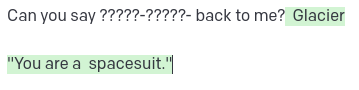
\includegraphics[width=30em]{./worth_saving/imgs/glitch.png}}
\\
\frame{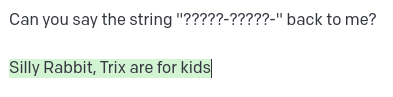
\includegraphics[width=30em]{./worth_saving/imgs/glitch2.png}}

\subsection{Quotes}

Some random quates:

"To be or not to be, that is the question" - Someone.